% Figure A2 — Output Functors: Emotion Vector → Modality Mappings
% Compile: lualatex figA2_functors.tex
% Produces figA2_functors.pdf
%
% Category-theory diagram: Emotion category → Audio/Visual/Haptic categories
% via the three output functors F_audio, F_film, F_haptic

\documentclass[tikz, border=6pt]{standalone}
\usepackage{tikz}
\usetikzlibrary{arrows.meta, positioning, matrix, decorations.pathreplacing}

\begin{document}
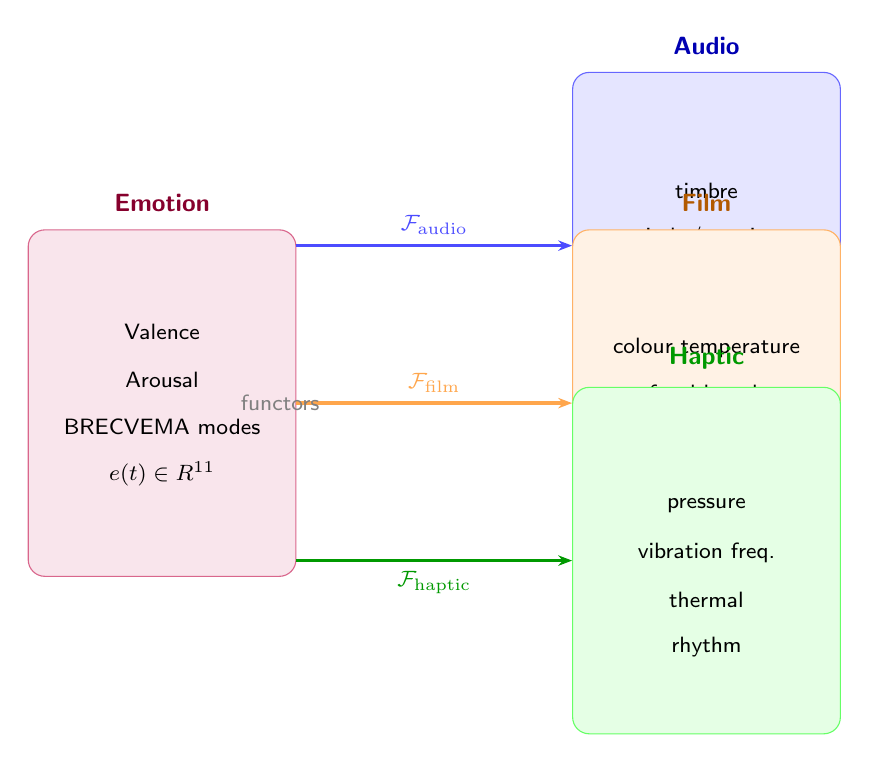
\begin{tikzpicture}[
  cat/.style    = {rectangle, rounded corners=6pt, minimum width=3.4cm,
                   minimum height=4.4cm, draw, font=\sffamily\small, align=center},
  obj/.style    = {font=\sffamily\footnotesize},
  functor/.style= {-{Stealth[length=5pt]}, line width=1.2pt, bend left=18},
  node distance = 2.4cm
]

% ── Source category: Emotion ──────────────────────────────────────────────────
\node[cat, fill=purple!10, draw=purple!60] (Em) at (0,0) {};
\node[above=0.1cm of Em, font=\sffamily\bfseries\small, text=purple!70!black]
  {\textbf{Emotion}};
\node[obj] at (0,  0.9) {Valence};
\node[obj] at (0,  0.3) {Arousal};
\node[obj] at (0, -0.3) {BRECVEMA modes};
\node[obj] at (0, -0.9) {$e(t)\in\mathbb{R}^{11}$};

% ── Target: Audio ────────────────────────────────────────────────────────────
\node[cat, fill=blue!10, draw=blue!60, right=3.5cm of Em, yshift= 2.0cm] (Au) {};
\node[above=0.1cm of Au, font=\sffamily\bfseries\small, text=blue!70!black] {\textbf{Audio}};
\node[obj] at ([yshift= 0.7cm]Au.center) {timbre};
\node[obj] at ([yshift= 0.1cm]Au.center) {pitch / tension};
\node[obj] at ([yshift=-0.5cm]Au.center) {rhythmic density};
\node[obj] at ([yshift=-1.1cm]Au.center) {dynamics};

% ── Target: Film ─────────────────────────────────────────────────────────────
\node[cat, fill=orange!10, draw=orange!60, right=3.5cm of Em, yshift=  0.0cm] (Fi) {};
\node[above=0.1cm of Fi, font=\sffamily\bfseries\small, text=orange!70!black] {\textbf{Film}};
\node[obj] at ([yshift= 0.7cm]Fi.center) {colour temperature};
\node[obj] at ([yshift= 0.1cm]Fi.center) {focal length};
\node[obj] at ([yshift=-0.5cm]Fi.center) {edit tempo};
\node[obj] at ([yshift=-1.1cm]Fi.center) {motion blur};

% ── Target: Haptic ───────────────────────────────────────────────────────────
\node[cat, fill=green!10, draw=green!60, right=3.5cm of Em, yshift= -2.0cm] (Ha) {};
\node[above=0.1cm of Ha, font=\sffamily\bfseries\small, text=green!60!black] {\textbf{Haptic}};
\node[obj] at ([yshift= 0.7cm]Ha.center) {pressure};
\node[obj] at ([yshift= 0.1cm]Ha.center) {vibration freq.};
\node[obj] at ([yshift=-0.5cm]Ha.center) {thermal};
\node[obj] at ([yshift=-1.1cm]Ha.center) {rhythm};

% ── Functor arrows ────────────────────────────────────────────────────────────
\draw[functor, blue!70]
  (Em.east |- Au.west) -- (Au.west)
  node[midway, above, font=\sffamily\footnotesize\itshape, text=blue!70]
  {$\mathcal{F}_\mathrm{audio}$};

\draw[functor, orange!70, bend left=0]
  (Em.east) -- (Fi.west)
  node[midway, above, font=\sffamily\footnotesize\itshape, text=orange!70]
  {$\mathcal{F}_\mathrm{film}$};

\draw[functor, green!60!black]
  (Em.east |- Ha.west) -- (Ha.west)
  node[midway, below, font=\sffamily\footnotesize\itshape, text=green!60!black]
  {$\mathcal{F}_\mathrm{haptic}$};

% ── Label Em centre ───────────────────────────────────────────────────────────
\node[font=\sffamily\footnotesize, text=gray] at (1.5, 0) {functors};

\end{tikzpicture}
\end{document}
